\documentclass[11pt,a4paper]{article}
\usepackage[spanish,es-nodecimaldot]{babel}	% Utilizar español
\usepackage[utf8]{inputenc}					% Caracteres UTF-8
\usepackage{graphicx}						% Imagenes
\usepackage[hidelinks]{hyperref}			% Poner enlaces sin marcarlos en rojo
\usepackage{fancyhdr}						% Modificar encabezados y pies de pagina
\usepackage{float}							% Insertar figuras
\usepackage[textwidth=390pt]{geometry}		% Anchura de la pagina
\usepackage[nottoc]{tocbibind}				% Referencias (no incluir num pagina indice en Indice)
\usepackage{enumitem}						% Permitir enumerate con distintos simbolos
\usepackage[T1]{fontenc}					% Usar textsc en sections
\usepackage{amsmath}						% Símbolos matemáticos
\usepackage{algorithm}						% Environtment algorithm
\usepackage[noend]{algpseudocode}			% Pseudocodigo
\usepackage{listings}

\algnewcommand\algorithmicforeach{\textbf{for each}}
\algdef{S}[FOR]{ForEach}[1]{\algorithmicforeach\ #1\ \algorithmicdo}

\algrenewcommand\algorithmicreturn{\textbf{return}}


\lstset{
	language=bash
}

% Comando para poner el nombre de la asignatura
\newcommand{\asignatura}{Metaheurísticas}
\newcommand{\autor}{Vladislav Nikolov Vasilev}

% Configuracion de encabezados y pies de pagina
\pagestyle{fancy}
\lhead{\autor{}}
\rhead{\asignatura{}}
\lfoot{Grado en Ingeniería Informática}
\cfoot{}
\rfoot{\thepage}
\renewcommand{\headrulewidth}{0.4pt}		% Linea cabeza de pagina
\renewcommand{\footrulewidth}{0.4pt}		% Linea pie de pagina

\begin{document}
\pagenumbering{gobble}

% Pagina de titulo
\begin{titlepage}

\begin{minipage}{\textwidth}

\centering

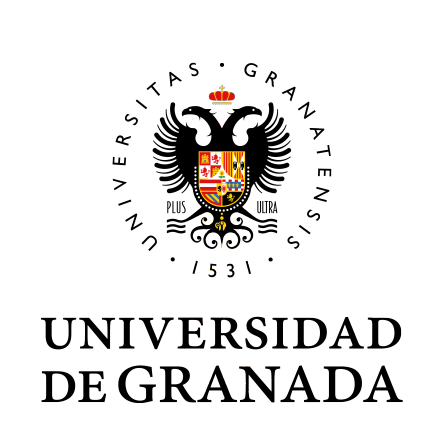
\includegraphics[scale=0.3]{img/ugr.png}\\

\textsc{\Large \asignatura{}\\[0.2cm]}
\textsc{GRADO EN INGENIERÍA INFORMÁTICA}\\[0.3cm]

\noindent\rule[-1ex]{\textwidth}{1pt}\\[1.5ex]
\textsc{{\Huge PRÁCTICA 3\\[1pt]}}
\textsc{{\Large \\Enfriamiento Simulado, Búsqueda Local Reiterada y Evolución Diferencial para el Problema del Aprendizaje de Pesos en Características}}
\noindent\rule[-1ex]{\textwidth}{2pt}\\[1ex]

\end{minipage}

\vspace{0.18cm}

\begin{minipage}{\textwidth}

\centering

\textbf{Autor}\\ {\autor{}}\\[1ex]
\textbf{NIE}\\ {X8743846M}\\[1ex]
\textbf{E-Mail}\\ {vladis890@gmail.com}\\[1ex]
\textbf{Grupo de prácticas}\\ {MH3 Jueves 17:30-19:30}\\[1ex]
\textbf{Rama}\\ {Computación y Sistemas Inteligentes}\\[1ex]
\vspace{0.2cm}


\includegraphics[scale=0.3]{img/etsiit.jpeg}

\vspace{0.3cm}
\textsc{Escuela Técnica Superior de Ingenierías Informática y de Telecomunicación}\\
\vspace{1cm}
\textsc{Curso 2018-2019}
\end{minipage}
\end{titlepage}

\pagenumbering{arabic}
\tableofcontents
\thispagestyle{empty}				% No usar estilo en la pagina de indice

\newpage

\setlength{\parskip}{1em}

\section{Descripción del problema}

El problema que se aborda en esta práctica es el Aprendizaje de Pesos en Características (APC). Es un problema típico de
\textit{machine learning} en el cuál se pretende optimizar el rendimiento de un clasificador basado en vecinos más cercanos.
Esto se consigue mediante la ponderación de las características de entrada con un vector de pesos $W$, el cuál utiliza
codificación real (cada $w_i \in W$ es un número real), con el objetivo de modificar sus valores a la hora de calcular la
distancia. Cada vector $W$ se expresa como $W = \lbrace w_1, w_2, \dots , w_n \rbrace$, siendo $n$ el número de dimensiones
del vector de características, y cumpliéndose además que $\forall w_i \in W, \; w_i \in [0, 1]$.\par

El clasificador considerado para este problema es el 1-NN (genéricamente, un clasificador $k$-NN, con $k$ vecinos, siendo
en este caso $k = 1$), es decir, aquél que clasifica un elemento según su primer vecino más cercano utilizando alguna medida
de distancia (en este caso, utilizando la distancia Euclídea). Cabe destacar que no en todos los casos se usará el clasificador
1-NN ya que se pueden dar casos en los que el vecino más cercano de un elemento sea él mismo. Por ese motivo, en algunas
técnicas/algoritmos se usará un 1-NN con el criterio de \textit{leave-one-out}, es decir, que se busca el vecino más cercano
pero excluyéndose a él mismo.\par

El objetivo propuesto es aprender el vector de pesos $W$
mediante una serie de algoritmos, de tal forma que al optimizar el clasificador se mejore tanto la precisión de éste como su
complejidad, es decir, que se considere un menor número de características. Estos dos parámetros, a los que llamaremos $tasa\_
clas$ y $tasa\_red$, respectivamente, se pueden expresar de la siguiente forma:

\[tasa\_clas = 100 \cdot \frac{nº \; instancias \; bien \; clasificadas \; en \; T}{nº \; instancias \; en \; T}\]
\[tasa\_red = 100 \cdot \frac{nº \; valores \; w_i < 0.2}{nº \; caracteristicas}\]

\noindent siendo $T$ el tamaño del conjunto de datos sobre que el que se evalúa el clasificador.\par

Por tanto, al combinarlos en una única función a la que llamaremos $F(W)$, la cuál será nuestra función objetivo a optimizar
(maximizar), tenemos que:

\[F(W) = \alpha \cdot tasa\_clas(W) + (1 - \alpha) \cdot tasa\_red(W)\] 

\noindent siendo $\alpha$ la importancia que se le asigna a la tasa de clasificación y a la de reducción, cumpliendo que
$\alpha \in [0, 1]$. En este caso, se utiliza un $\alpha = 0.5$ para dar la misma importancia a ambos, con lo cuál se pretende
que se reduzcan al máximo el número de características conservando una $tasa\_clas$ alta.

\section{Descripción de los algoritmos}

\subsection{Consideraciones previas}

Antes de empezar con la descripción formal de los algoritmos implementados, vamos a describir algunos aspectos
comunes, como por ejemplo cómo se representan e inicializan las soluciones en todos los casos, cómo se representa la función
objetivo o \textit{fitness} y cómo se evalúan las soluciones. También vamos a comentar brevemente otros aspectos, como por
ejemplo cómo mantener las soluciones factibles después de aplicarles alguna mutación o transformación (es decir, que se
mantengan en el rango dado), entre otros.
Cabe destacar que muchos de los pseudocódigos que aparecen a continuación no se han implementado exactamente igual o no aparecen
en el código, ya que o bien son operaciones que se han vectorizado o bien ya hay funciones que hacen eso.

Como se dijo al principio, cada solución es un vector de valores reales $W$ en el que $\forall w_i \in W, \; w_i \in [0, 1]$.
En el caso de la \textbf{Evolución Diferencial} se tendrá un conjunto vectores que formarán la población, ya que sigue un esquema
basado en poblaciones. Esto se volverá a comentar más adelante, cuando se hable con más detenimiento de esta técnica.

Para evitar que las soluciones se salgan de este intervalo, se ha implementado una función que se encarga de normalizar los valores
de $W$ en el rango. La función se ha usado, por ejemplo, en la búsqueda local, para hacer que al aplicar el operador
de generación de un nuevo vecino la solución siguiese siendo válida. La implementación de esta función es la siguiente:

\begin{algorithm}[H]
\caption{Función que normaliza un vector de pesos $W$}
\begin{algorithmic}[1]
\Function{NormalizarW}{$W$}
\ForEach{$w_i \in W$}
	\If{$w_i < 0$}
		\State $w_i \gets 0$
	\ElsIf{$w_1 > 1$}
		\State $w_i \gets 1$
	\EndIf
\EndFor
\State \Return{$W$}
\EndFunction
\end{algorithmic}
\end{algorithm}

Para generar las soluciones iniciale se han seguido dos esquemas. En uno de ellos, el cuál es utilizado por el \textbf{Enfriamiento
Simulado} y la \textbf{ILS}, se genera un único vector de pesos inicial con valores aleatorios dados por una distribución uniforme
en el rango $[0, 1]$. En el otro esquema, el cuál es seguido por la \textbf{Evolución Diferencial} se lleva a cabo algo muy parecido,
solo que en vez de generar una única solución inicial, se generan una serie de $M$ soluciones iniciales, donde $M$ es el tamaño de
la población. Los pseudocódigos de estos dos esquemas se pueden ver a continuación:

\begin{algorithm}[H]
\caption{Inicialización de un vector de pesos $W$}
\begin{algorithmic}[1]
\Function{GenerarWAleatorio}{$N$}
\State$W \gets$ vector[$N$]
\ForEach{$w_i \in W$}
	 \State $w_i \gets$ ValorAleatorioUniformeRango0-1()
\EndFor
\State \Return{$W$}
\EndFunction
\end{algorithmic}
\end{algorithm}

\begin{algorithm}[H]
\caption{Generación de una población inicial en \textbf{Evolución Diferencial}}
\begin{algorithmic}[1]
\Function{GenerarPoblacionInicial}{$numCrom$, $numGenes$}
\State $poblacion \gets $ NuevaMatrizVacia($numCrom$, $numGenes$)
	\For{$i \gets 0$ \textbf{to} $numCrom - 1$}
		\For{$j \gets 0$ \textbf{to} $numGenes- 1$}
			\State $poblacion[i][j] \gets $ ValorAleatorioUniformeRango0-1()
		\EndFor	
	\EndFor
\State \Return{$poblacion$}
\EndFunction
\end{algorithmic}
\end{algorithm}

Vamos a comentar ahora algunos detalles extra. Es importante saber como se calcula la distancia a un vecino, ya que esto juega
un factor muy importante a la hora de encontrar cuál es el vecino más cercano a un elemento (o el vecino más cercano por el
criterio \textit{leave-one-out}). En la implementación de la práctica se ha utilizado un KDTree, que es una estructura de datos
parecida a un árbol binario, solo que de $K$ dimensiones. Por dentro, esta estructura utiliza la distancia Euclídea (distancia
en línea recta entre dos elementos) para determinar cuál es el elemento más próximo a otro. No hace falta conocer como se
implementa esta estructura de datos, pero sí es importante conocer cómo se realiza el cálculo de la distancia Euclídea. En el
siguiente pseudocódigo se puede ver el cálculo:

\begin{algorithm}[H]
\caption{Cálculo de la distancia Euclídea entre dos puntos}
\begin{algorithmic}
\Function{DistanciaEuclidea}{$e_1, e_2$}
\State $distancia \gets \sqrt{\sum_{i=1}^{N} (e_1^i - e_2^i)^2}$
\State \Return{$distancia$}
\EndFunction
\end{algorithmic}
\end{algorithm}

Para la \textbf{Evolución Diferencial} sería interesante intentar mantener la población ordenada por valor \textit{fitness}, ya que
eso nos va a simplificar bastante el trabajo para uno de los procesos de mutación. Para hacer esto, se ha creado una función que
recibe la lista de valores \textit{fitness} y la poblacion, obtiene los índices que dan el orden de forma ascendente de la lista
y con estos índices ordena la población y la lista de \textit{fitness}. Aquí se puede ver como funciona:

\begin{algorithm}
\caption{Función para ordenar la población según su valor \textit{fitness}}
\begin{algorithmic}[1]
\Function{OrdenarPoblacion}{$fitness$ , $poblacion$}
\State $indicesOrden \gets $ ObtenerIndicesOrdenados($fitness$)
\State $fitnessOrdenado \gets$ NuevoVectorVacioMismaCapacidad($fitness$)
\State $poblacionOrdenada \gets$ NuevaMatrizVaciaMismaCapacidad($poblacion$)
\ForEach{$indice \in indicesOrden$}
	\State $fitnessOrdenado \gets fitness[indice]$
	\State $poblacionOrdenada \gets poblacion[indice]$
\EndFor
\State \Return{$fitnessOrdenado$, $poblacionOrdenada$}
\EndFunction
\end{algorithmic}
\end{algorithm}

Pasemos a ver ahora la función objetivo, $F(W)$, que es lo que se pretende optimizar. Para evaluar la función objetivo,
necesitamos calcular $tasa\_clas$ y $tasa\_red$. Para calcular lo primero, podemos seguir la idea detrás del siguiente
pseudocódigo:

\begin{algorithm}[H]
\caption{Cálculo de la tasa de clasificación}
\begin{algorithmic}[1]
\Function{CalculoTasaClas}{$etiq, etiqPred, N$}
\State $bienClasificados \gets 0$
\For{$i \gets 1$ \textbf{to} $N$}
	\If{$etiq_i = etiqPred_i$}
		\State $bienClasificados \gets bienCasificados + 1$
	\EndIf
\EndFor
\State $tasa\_clas \gets bienClasificados$ / $N$
\State \Return{$tasa\_clas$}
\EndFunction
\end{algorithmic}
\end{algorithm}

Para calcular $tasa\_red$, suponiendo que queremos saber el número de características por debajo de $0.2$ podemos seguir un
esquema como el siguiente:

\begin{algorithm}[H]
\caption{Cálculo de la tasa de reducción (I)}
\begin{algorithmic}[1]
\Function{CalculoTasaRed}{$W, N$}
\State $caracRed \gets 0$
\ForEach{$w_i \in W$}
	\If{$w_i < 0.2$}
		\State $caracRed \gets caracRed + 1$
	\EndIf
\EndFor
\State $tasa\_red \gets caracRed$ / $N$
\State \Return{$tasa\_red$}
\EndFunction
\end{algorithmic}
\end{algorithm}

Y finalmente, para poder calcular la función a optimizar (nuestra función \textit{fitness} u objetivo), teniendo en cuenta que
usamos un $\alpha = 0.5$ para ponderar las dos tasas, y que anteriormente hemos calculado ambas tasas, podemos seguir el
siguiente esquema:

\begin{algorithm}[H]
\caption{Cálculo de la función objetivo o \textit{fitness}}
\begin{algorithmic}[1]
\Function{CalculoFuncionFitness}{$tasa\_clas, tasa\_red, \alpha$}
\State $fitness \gets \alpha \cdot tasa\_clas + (1 - \alpha) \cdot tasa\_red$
\State \Return{$fitness$}
\EndFunction
\end{algorithmic}
\end{algorithm}

Para acabar, y antes de pasar a ver la implementación de los algoritmos, veamos otra funcionalidad que se usa en todos los
algoritmos, que es la forma en la que se evalúa la función objetivo. Podemos evaluar la función objetivo tanto para una solución
como para una población de soluciones. Por tanto, vamos a tener dos funciones que nos permitan evaluar las soluciones: una para
una única solución y una para toda una población de individuos (soluciones), la cuál por debajo utilizará la evaluación simple
tantas veces como individuos tenga la población. Vamos a ver el funcionamiento de estas funciones comenzando primero por
la que evalúa una única solución, y veamos luego la función que evalúa toda una población de soluciones:

\begin{algorithm}[H]
\caption{Función para evaluar un vector de pesos $W$}
\begin{algorithmic}[1]
\Function{Evaluar}{$datos$, $etiquetas$, $W$}
\State $datosPesos \gets$ aplicar $w_i \in W$ sobre los $x_i \in datos$ donde $w_i > 0.2$
\State $arbolKD \gets$ KDTree($datosPesos$)
\State $vecinos \gets arbolKD$.ObtenerVecinosMasCercanoL1O($datosPesos$)
\State $pred \gets etiquetas[vecinos]$
\State $tasa\_clas \gets$ CalcularTasaClas($etiquetas$, $pred$, num. etiquetas)
\State $tasa\_red \gets$ CalcularTasaRed($W$, num. caracteristicas)
\State $fitness \gets$ CalculoFuncionFitness($tasa\_clas$, $tasa\_red$)
\State \Return{$fitness$}
\EndFunction
\end{algorithmic}
\end{algorithm}

\begin{algorithm}[H]
\caption{Función para evaluar una población}
\begin{algorithmic}[1]
\Function{EvaluarPoblacion}{$datos$, $etiquetas$, $poblacion$}
\State $listaFitness \gets $ NuevoVector()
\ForEach{$W \in poblacion$}
	\State $listaFitness$.Añadir(Evaluar($datos$, $etiquetas$, $W$))
\EndFor
\State \Return{$listaFitness$}
\EndFunction
\end{algorithmic}
\end{algorithm}

\newpage

\subsection{Algoritmos de comparación}

\subsubsection{Clasificador 1-NN}

El primer algoritmo con el que compararemos es el 1-NN que utiliza todas las características, tal como hacíamos en la 
práctica anterior.

Este clasificador lo que hace es, dado un conjunto de valores $X$ que pertenecen a una muestra y un elemento $e$, decir cuál es el
$x \in X$ más cercano a $e$, y por tanto, decir que $e$ pertenece a la misma clase $x$. Para determinar cuál es el elemento más
cercano se puede usar alguna métrica de distancia, como por ejemplo la distancia Euclídea, descrita anteriormente. A la hora de
implementarlo, para poder acelerar los cálculos, se puede usar un KDTree, ya que permite realizar una consulta rápida (en los
casos más favorables su complejidad temporal es $\mathcal{O} (\log n)$, mientras que en el peor caso es $\mathcal{O}(n)$)
utilizando la distancia Euclídea para determinar el vecino más cercano, con la penalización de que tarda un tiempo
$\mathcal{O}(n)$ en ser construido. Para poder ver un esquema de su funcionamiento, se ofrece el siguiente pseudocódigo:

\begin{algorithm}[H]
\caption{Clasificador 1-NN}
\begin{algorithmic}[1]
\Function{KNN}{$X$, $y$, $e$}
\State $arbolKD \gets$ KDTree($X$)
\State $x \gets arbolKD$.VecinoMasCercano($e$)
\State $etiqueta \gets y[x]$
\State \Return{$etiqueta$}
\EndFunction
\end{algorithmic}
\end{algorithm}

\newpage

\subsubsection{Algoritmo greedy \textit{RELIEF}}

Otro algoritmo con el que vamos a comparar es el algoritmo para el cálculo de pesos \textit{RELIEF}. Es un algoritmo
greedy que, comenzando con un $W$ cuyos pesos valen 0, actualiza $W$ para cada $x_i \in X$, buscando para cada $x_i$ cuál es
su aliado más cercano (elemento que tiene la misma etiqueta que $x_i$ con el criterio de \textit{leave-one-out}, ya que él
mismo podría ser su vecino más cercano) y su enemigo más cercano (elemento que tiene diferente etiqueta a la que tiene $x_i$).

A la hora de implementarlo, vamos a utilizar 2 KDTree en cada iteración que se van a construir sobre la marcha. En uno se
encontrarán todos los aliados de $e$ y en el otro estarán todos sus enemigos. Esto puede suponer una gran penalización por el
tiempo de creación de los árvoles, pero es un tiempo insignificante ya que el algoritmo es muy rápido. Después de construir los
árboles, se buscará en el caso del aliado más cercano, por el criterio de \textit{leave-one-out}, cuál es el índice de este
aliado. En el caso del enemigo más cercano, como este no puede ser él mismo, se buscará el índice del vecino más cercano en ese
árbol. Una vez hecho eso, obtendremos los respectivos aliado y enemigo del conjunto de aliados y enemigos. Una vez teniéndolos,
ya se puede actualizar el valor de $W$.

Cuando se ha terminado de iterar sobre todos los elementos de $X$, se normaliza $W$ para que esté en el rango $[0, 1]$ 
eligiendo el $w_i \in W$ que sea más grande. Todos aquellos valores por debajo de 0 se truncan a 0, y el resto se normaliza
dividiéndolos entre $w_m$ (el $w_i$ más grande).

Antes de ver su implementación, veamos como se inicializa una solución:

\begin{algorithm}[H]
\caption{Inicialización de un vector de pesos $W$ en \textit{RELIEF}}
\begin{algorithmic}[1]
\Function{GenerarWRelief}{$N$}
\State $W \gets$ VectorVacioCapacidad($N$)
\ForEach{$w_i \in W$}
	\State $w_i \gets 0$
\EndFor
\State \Return{$W$}
\EndFunction
\end{algorithmic}
\end{algorithm}

Una vez dicho esto, veamos cómo sería la implementación:

\begin{algorithm}[H]
\caption{Cálculo de los pesos mediante \textit{RELIEF} (I)}
\begin{algorithmic}[1]
\Function{RELIEF}{$X$, $Y$}
\State $N \gets$ ObtenerNumElementos($Y$)
\State $numCarac \gets $ ObtenerNumCarac($X$)
\State $W \gets $ GenerarWRelief($numCarac$)
\algstore{relief}
\end{algorithmic}
\end{algorithm}

\begin{algorithm}[H]
\caption{Cálculo de los pesos mediante \textit{RELIEF} (II)}
\begin{algorithmic}
\algrestore{relief}
\For{$i \gets 0$ \textbf{to} $N-1$}
	\State $x, y \gets X[i], Y[i]$
	\State $aliados \gets e_a \subset X :$ etiqueta($e_a$) $ = y$
	\State $enemigos \gets e_e \subset X:$ etiqueta($e_e$) $ \neq y$
	\State $arbolAliados \gets$ KDTree($aliados$)
	\State $arbolEnemigos \gets$ KDTree($enemigos$)
	\State $aliadoCercano \gets arbolAliados$.ObtenerVecinoMasCercanoL1O($x$)
	\State $enemigoCercano \gets arbolEnemigos$.ObtenerVecinoMasCercano($x$)
	\State $aliado \gets aliados[aliadoCercano]$
	\State $enemigo \gets enemigos[enemigoCercano]$
	\State $W \gets W + \left|x - enemigo\right| - \left|x - aliado\right|$
\EndFor
\State $w_m \gets$ \textbf{max}($W$)
\ForEach{$w_i \in W$}
	\If{$w_i < 0$}
		\State $w_i \gets 0$
	\Else
		\State $w_i \gets w_i$ / $w_m$
	\EndIf
\EndFor
\State \Return{$W$}
\EndFunction
\end{algorithmic}
\end{algorithm}

\newpage

\subsubsection{Búsqueda Local}
\label{subsubsect:ls}

En la primera práctica se implementó una búsqueda local (búsqueda basada en trayectorias), así que vamos a rescatarla para
tener un algoritmo más de comparación, ademñas de que los AM la necesitarán luego, aunque ligeramente modificada. Esta búsqueda,
como debemos recordar, está basada en el primer mejor (Simple Hill Climbing).

La búsqueda local parte de un vector $W$ con valores aleatorios y busca optimizarlo mediante la exploración de los vecinos.
Esta exploración se realiza modificando con un valor aleatorio generado a partir de una distribución normal con $\mu = 0$ y 
$\sigma = 0.3$ un $w_i \in W$, quedándose con el cambio en caso de mejorar la función objetivo, o descartándolo en otro caso.

Para realizar lo explicado anteriormente, se genera una permutación del conjunto $\lbrace 0, 1, \dots , N-1 \rbrace$, donde $N$
es el número de características, y se van escogiendo las características según el orden de la permutación, aplicándoles
el cambio anteriormente descrito. Si no se produce una mejora, se descarta el cambio realizado. Si no se ha producido mejora
en la función objetivo con la permutación, se escoge una nueva permutación y se repite el proceso, hasta un máximo de $20
\cdot N$ evaluaciones sin éxito seguidas de la función objetivo. Si se produce mejora, se acepta el cambio y se genera una
nueva permutación, repitiendo el proceso. Todo esto se realiza hasta que se hayan realizado 15000 evaluaciones de la función
objetivo, o hasta que se dé la condición anterior (demasiadas iteraciones sin mejora).

El pseudocódigo de la búsqueda local se puede ver aquí:

\begin{algorithm}[H]
\label{alg:local-search}
\caption{Cálculo de los pesos mediante la Búsqueda Local (I)}
\begin{algorithmic}[1]
\Function{BusquedaLocal}{$datos$, $etiquetas$}
\State $N \gets $ ObtenerNumCaracteristicas($datos$)
\State $W \gets$ GenerarWAleatorio($N$)
\State $evaluaciones \gets 0$
\State $evaluacionesMalas \gets 0$
\State $fitness \gets$ Evaluar($datos$, $etiquetas$, $W$)
\While{$evaluaciones < 15000$}
\State $Wactual \gets W$
\State $ordenCaracteristicas \gets $ Permutacion(0 \textbf{to} $N - 1$)
\ForEach{$carac \in ordenCaracteristicas$}
	\State $W[carac] \gets W[carac] + $ GenerarValorDistribucionNormal($\mu$, $\sigma$)	
	\State $W \gets$ NormalizarW($W$)
	\State $evaluaciones \gets evaluaciones + 1$
	\State $nuevoFitness \gets$ Evaluar($X, Y, W$)		
\algstore{local}
\end{algorithmic}
\end{algorithm}

\begin{algorithm}[H]
\caption{Cálculo de los pesos mediante la Búsqueda Local (II)}
\begin{algorithmic}
\algrestore{local}
	\If{$nuevoFitness > fitness$}
		\State $fitness \gets nuevoFitness$		
		\State $evaluacionesMalas \gets 0$		
		\State \textbf{break}
	\Else
		\State $evaluacionesMalas \gets evaluacionesMalas + 1$		
		\State $W[carac] \gets Wactual[carac]$		
	\EndIf	
	\If{$evaluaciones > 15000$ \textbf{or} $evaluacionesMalas > 20 \cdot N$}
		\State \Return{$W$}
	\EndIf
\EndFor
\EndWhile
\State \Return{$W$}
\EndFunction
\end{algorithmic}
\end{algorithm}

\newpage

\subsection{Algoritmos implementados}

\subsubsection{Enfriamiento Simulado}

La primera técnica que se ha implementado en esta práctica es el \textbf{Enfriamiento Simulado}. Esta es una búsqueda basada
en trayectorias que se inspira en la termodinámica. Esta técnica, al igual que la Búsqueda Local, explora el entorno de la
solución actual con el objetivo de intentar encontrar una solución mejor. Sin embargo, a diferencia de esta última, el
\textbf{Enfriamiento Simulado} puede seleccionar soluciones peores que la actual con una cierta probabilidad, la cuál tendrá en
cuenta a la temperatura. A mayor temperatura, mayor será la posibilidad de aceptar una solución peor, y a menor temperatura,
menor probabilidad de hacerlo. Por tanto, es una técnica que permite explorar más al principio, ya que al aceptar soluciones
peores se pueden salir por ejemplo de zonas de óptimos locales, mientras que al final permite explotar más, ya que habrá menos
probabilidad de aceptar una solución que empeore a la actual.

El esquema de enfriamiento que sigue este algoritmo es el \textbf{esquema modificado de Cauchy}, el cuál permitirá realizar
enfriamientos de forma proporcional a un parámetro $\beta$. Este esquema se puede ver en el siguiente pseudocódigo:

\begin{algorithm}[H]
\caption{Esquema de enfriamiento de Cauchy modificaco}
\begin{algorithmic}[1]
\Function{EsquemaCauchyModificado}{$T_K, \beta$}
\State $T_{K+1} \gets T_K$ / $(1 + \beta \cdot T_K)$
\State \Return{$T_{K+1}$}
\EndFunction
\end{algorithmic}
\end{algorithm}

El valor de $\beta$ depende de la temperatura inicial, de la temperatura final que se quiere alcanzar y de un valor $M$, que es
el número de enfriamientos que se quieren hacer. Esto se puede ver en el siguiente pseudocódigo:

\begin{algorithm}[H]
\caption{Cálculo del valor de $\beta$}
\begin{algorithmic}[1]
\Function{CalcularBeta}{$T_0$, $T_f$, $M$}
\State $\beta \gets (T_0 - T_f)$ / $(M \cdot T_0 \cdot T_f)$
\State \Return{$\beta$}
\EndFunction
\end{algorithmic}
\end{algorithm}

La temperatura inicial se ha especificado que se calcule de la siguiente forma, donde $C$ es el coste de la solución inicial y
$\phi \in [0, 1]$ es la probabilidad de aceptar un $\mu$ por 1 peor que la inicial. Se ha especificado en este problema que
$\phi = 0.3$ y que $\mu = 0.3$.

\begin{algorithm}[H]
\caption{Cálculo de la temperatura inicial}
\begin{algorithmic}[1]
\Function{CalcularTempInicial}{$C$, $\mu$, $\phi$}
\State $T_0 \gets (\mu \cdot C)$ / $-\ln (\phi)$
\State \Return{$T_0$}
\EndFunction
\end{algorithmic}
\end{algorithm}

También es importante saber como se generan los vecinos de una solución. Para ello, hace falta modificar una característica
aleatoria del vector de pesos añadiéndole un valor aletorio generado mediante una distribución normal de $\mu = 0$ y $\sigma = 0.3$.
Es importante destacar que este vecino tiene que normalizarse después de añadirle el valor aleatorio, ya que se tiene que dar que
$\forall w_i \in W$, $w_i \in [0, 1]$. Esto se puede ver en el siguiente pseudocódigo:

\begin{algorithm}[H]
\caption{Operador de generación de vecino}
\begin{algorithmic}[1]
\Function{OperadorVecindario}{$W$, $N$}
\State $carac \gets$ ValorEnteroAleatorio($N$)
\State $vecino[carac] \gets vecino[carac] + $ GenerarValorDistribucionNormal($\mu$, $\sigma$)
\State NormalizarW($vecino$)
\State \Return{$vecino$}
\EndFunction
\end{algorithmic}
\end{algorithm}

Antes de ver finalmente el pesudocódigo del Enfriamiento Simulado, hace falta comentar unos aspectos muy breves sobre él. Se ha
especificado que el \textbf{número máximo de evaluaciones} sea 15000. Además, se ha modificado el bucle externo para que se hagan
$M$ iteraciones, siempre y cuando ha habido algún éxito, que es entrar dentro del bloque condicional, debido a que se ha encontrado
una solución mejor o se ha aceptado una peor con una cierat probabilidad dada por un valor aleatorio uniforme en el rango $[0, 1]$.
Y otra cosa importante es que, ya que estamos en un problema de maximización, el valor de $\Delta f$ tiene que ser positivo, y
al ser este valor positivo, dentro de la exponencial se tiene que eliminar el signo negativo que viene en la versión original.

Con esto ya dicho, pasemos a ver finalmente el pseudocódigo de esta técnica:

\begin{algorithm}[H]
\caption{Función de cálculo de pesos mediante Enfriamiento Simulado (I)}
\begin{algorithmic}[1]
\Function{EnfriamientoSimulado}{$X$, $y$, $maxEvaluaciones$}
\State $T_f \gets 0.001$
\State $N \gets $ ObtenerNumCaracteristicas($X$)
\State $W \gets $ GenerarWAleatorio($N$)
\State $mejorW \gets W$
\State $maxVecinos \gets 10 \cdot N$
\State $maxExitos \gets $ Redondear($0.1 \cdot maxVecinos$)
\State $M \gets $ Redondear($maxEvaluaciones$ / $maxVecinos$)
\algstore{sa}
\end{algorithmic}
\end{algorithm}

\begin{algorithm}[H]
\caption{Función de cálculo de pesos mediante Enfriamiento Simulado (II)}
\begin{algorithmic}
\algrestore{sa}
\State $numEvaluaciones \gets 0$
\State $numIteraciones \gets 0$
\State $numExitos \gets 1$
\State $C \gets $ Evaluar($X$, $y$, $W$)
\State $mejorFitness \gets C$
\State $fitness \gets C$
\State $numEvaluacions \gets numEvaluaciones + 1$
\State $T \gets $ CalcularTempInicial($C$, $\mu$, $\phi$)
\State $\beta \gets $ CalcularBeta($T$, $T_f$, $M$)
\While{$numIteraciones < M$ \textbf{and} $numExitos > 0$}
	\State $numExitos \gets 0$
	\State $numVecinos \gets 0$
	\While{$numVecinos < maxVecinos$ \textbf{and} $numExitos < maxExitos$}
		\State $W' \gets $ OperadorVecindario($W$, $N$)
		\State $fitness' \gets $ Evaluar($X$, $y$, $W'$)
		\State $numEvaluaciones \gets numEvaluaciones + 1$
		\State $\Delta f \gets fitness' - fitness$
		\If{$\Delta f > 0$ \textbf{or} ValorAleatorioUniformeRango0-1() $\leq e^{\Delta f \; / \; T}$}
			\State $numExitos \gets numExitos + 1$
			\State $W \gets W'$
			\State $fitness \gets fitness'$
			\If{$fitness > mejorFitness$}
				\State $mejorW \gets W$
				\State $mejorFitness \gets fitness$
			\EndIf
		\EndIf	
		\State $numVecinos \gets numVecinos + 1$
	\EndWhile
	\State $T \gets$ EsquemaCauchyModificado($T$, $\beta$)
	\State $numIteraciones \gets numIteraciones + 1$	
\EndWhile
\State \Return $mejorW$
\EndFunction
\end{algorithmic}
\end{algorithm}

\newpage

\subsubsection{ILS: Búsqueda Local Iterativa}

La segunda técnica que se ha implementado es la \textbf{ILS}, o como se conoce en español, \textbf{Búsqueda Local Iterativa}.
Esta es una búsqueda basada en trayectorias que, a diferencia de la búsqueda local, permite evitar óptimos locales, reiniciando
la búsqueda con una nueva solución inicial. Se parte de una solución inicial y se aplica una búsqueda local sobre ella, y el
restultado se guarda como la mejor solución hasta el momento. A continuación se aplica una mutación sobre la mejor solución
actual, modificando una parte de los valores de la solución y se vuelve a aplicar una búsqueda local sobre esta modificación.
aceptando no esta nueva solución como la mejor actual según algún criterio, y se repite este proceso hasta que se dé un cierto 
de parada.

En este problema, el operador de mutación que se aplica sobre la soluión modifica un 10\% de las características de forma aleatoria
añadiéndoles un valor aleatorio generado por una distribución normal de $\mu = 0$ y $\sigma = 0.4$. Esto se puede ver en el
siguiente pseudocódigo:

\begin{algorithm}[H]
\caption{Operador de mutación en ILS}
\begin{algorithmic}[1]
\Function{Mutacion}{$W$, $N$}
\State $caracteristicas \gets $ GenerarSecuenciaAleatoriaEnteros($N$, $0.1$)
\For{$carac \in caracteristicas$}
	\State $W[carac] \gets W[carac] + $ GenerarValorDistribucionNormal($\mu$, $\sigma$)
\EndFor
\State $W \gets$ NormalizarW($W$)
\State \Return{$W$}
\EndFunction
\end{algorithmic}
\end{algorithm}

En este problema, se piden hacer de nuevo 15000 evaluaciones de la función objetivo. Además, se utiliza la búsqueda local
de la sección \ref{subsubsect:ls}, modificándola para que acepte un número máximo de iteraciones de 1000 (que es el número
de evaluaciones que se pide que haga la búsqueda local) y un vector de pesos de entrada, de forma que no tiene que generarlo
ella, aunque sí que debe evaluarlo. Además, se elimina toda la parte que implica parar antes de tiempo por no mejorar. También
se hace que devuelva el \textit{fitness} de la solución a la que ha llegado, para así evitar tener que volver a calcularlo
posteriormente. A continuación se puede ver un pseudocódigo del ILS:

\begin{algorithm}[H]
\caption{Cálculo de los pesos mediante la ILS (I)}
\begin{algorithmic}[1]
\Function{ILS}{$X$, $y$, $maxEvaluaciones$}
\State $N \gets$ ObtenerNumCaracteristicas($X$)
\State $numEvaluaciones \gets 0$
\State $evalsBL \gets 1000$
\State $W_0 \gets$ GenerarWAleatorio($N$)
\algstore{ils}
\end{algorithmic}
\end{algorithm}

\begin{algorithm}[H]
\caption{Cálculo de los pesos mediante la ILS (II)}
\begin{algorithmic}
\algrestore{ils}
\State $mejorW, mejorFitness \gets$ BusquedaLocal($X$, $y$, $W_0$, $evalsBL$)
\State $numEvaluaciones \gets numEvaluaciones + evalsBL$
\While{$numEvaluaciones < maxEvaluaciones$}
	\State $W' \gets mejorW$
	\State $W' \gets $ Mutacion($W'$, $N$)
	\State $W', fitness \gets$ BusquedaLocal($X$, $y$, $W'$, $evalsBL$)
	\If{$fitness > mejorFitness$}
		\State $mejorW \gets W'$
		\State $mejorFitness \gets fitness$
	\EndIf
\EndWhile
\State \Return{$mejorW$}
\EndFunction
\end{algorithmic}
\end{algorithm}

\newpage

\subsubsection{Evolución Diferencial}

La tercera y última técnica que se ha pedido implementar es la \textbf{Evolución Diferencial}. Esta es una metaheurística basada
en poblaciones, al igual que los Algoritmos Genéticos. Sin embargo, esta técnica está especialmente diseñada para problemas
con variables reales, ya que las mutaciones y recombinaciones están especialmente pensados para éstos. Estos operadores permiten
combinar tanto la capacidad explorativa de los AG como su capacidad explotativa con tal de conseguir unos mejores resultados.

En este problema se utilizan dos mutaciones. Una de ellas es el \textit{Rand}, donde se escogen 3 padres aleatorios y se
combinan entre ellos. El otro es el \textit{current-to-best/1}, donde se escogen dos padres aleatorios, el mejor elemento
de la población y el elemento $i$-ésimo sobre el que se está haciendo la mutación, y se combinan entre ellos. Esto se puede ver
en los siguientes pseudocódigos:

\begin{algorithm}[H]
\caption{Esquema de mutación \textit{Rand}}
\begin{algorithmic}[1]
\Function{MutacionRand}{$p1$, $p2$, $p3$, $f$ $gen$}
\State $mutacion \gets p1[gen] + f (p2 - p3)$
\State \Return{$mutacion$}
\EndFunction
\end{algorithmic}
\end{algorithm}

\begin{algorithm}[H]
\caption{Esquema de mutación \textit{current-to-best/1}}
\begin{algorithmic}[1]
\Function{MutacionCurrentToBest}{$mejor$, $actual$, $p1$, $p2$, $f$ $gen$}
\State $mutacion \gets mejor[gen] + f (mejor[gen] - actual[gen]) + f (p1[gen] - p2[gen])$
\State \Return{$mutacion$}
\EndFunction
\end{algorithmic}
\end{algorithm}

Esta mutación, sin embargo, no se hace siempre, si no que viene por una tasa de cruce ($CR$). Se genera un número aleatorio y,
en caso de obtener un valor más pequeño que $CR$, de realiza la mutación en el gen. En caso contrario, se copia la información
genética del cromosoma sobre el que se están realizando las operaciones.

Una vez que se han generado todos los descendientes, éstos tienen que competir contra sus padres directos. Los descendientes
solo pueden entrar en la población si su valor \textit{fitness} es mejor que el de sus padres. En caso contrario, serán ignorados.

Para facilitar un poco el trabajo, la población estará ordeanda según su valor \textit{fitness}, ya que uno de los modelos de
mutación utiliza el mejor cromosoma. Por tanto, para tener un acceso más rápido a él, lo más adecuado sería tener toda la población
ordenada.

Para este problema se tienen que realizar de nuevo 15000 evaluaciones a la función objetivo. Los valores de $CR$ y $f$ son
ambos 0.5, con lo cuál hay bastante probabilidad de cruce.

Con todo esto dicho, vamos a ver un pseudocódigo de la Evolución Diferencial:

\begin{algorithm}[H]
\caption{Evolución Diferencial}
\begin{algorithmic}[1]
\Function{AGG}{$X$, $Y$, $opMutacion$}
\State $numGenes \gets$ ObtenerNumCaracteristicas($datos$)
\State Determinar $numPadres$ en función de $opMutacion$
\State $numEvaluaciones \gets 0$
\State $poblacion \gets$ GenerarPoblacionInicial($numCrom$, $numGenes$)
\State $fitness \gets$ EvaluarPoblacion($datos$, $etiquetas$, $poblacion$)
\State $fitness$, $poblacion \gets$ OrdenarPoblacion($fitness$, $poblacion$)
\State $numEvaluaciones \gets numEvaluaciones + tamPob$
\While{$numEvaluaciones < 15000$}
	\State $descendientes \gets$ NuevoVectorVacio()
	\For{$i \gets 1$ \textbf{to} $tamPob$}
		\State $indicesPadres \gets$ GenerarIndicesExcluyendoValorI($N$, $i$)
		\State Escoger $numPadres$ de $indicesPadres$ de forma aleatoria
		\State $descendiente \gets$ NuevoVectorVacio()
		\For{$gen \gets 1$ \textbf{to} $numGenes$}
			\If{GenerarValorAleatorioUniforme01() $< CR$}
				\State $descendiente[gen] \gets$ Aplicar mutación según $opMutacion$
			\Else{}
				\State $descendiente[gen] \gets poblacion[i][gen]$
			\EndIf
		\EndFor
		\State $descendiente \gets$ NormalizarW($descendiente$)
		\State $descendientes$.Insertar($descendiente$)
	\EndFor
	\State $fitnessDesc \gets$ EvaluarPoblacion($X$, $y$, $descendientes$)
	\State $numEvaluaciones \gets numEvaluaciones + numCrom$
	\For{$i \gets 1$ \textbf{to} $tamPob$}
		\If{$fitnessDesc[i] > fitness[i]$}
			\State $poblacion[i] \gets descendientes[i]$
			\State $fitness[i] \gets fitnessDesc[i]$
		\EndIf
	\EndFor
	\State $fitness$, $poblacion \gets$ OrdenarPoblacion($fitness$, $poblacion$)
\EndWhile
\State $W \gets poblacion[0]$
\State \Return{$W$}
\EndFunction
\end{algorithmic}
\end{algorithm}

\newpage

\section{Desarrollo de la práctica}

La práctica se ha implementado en \textbf{Python3} y ha sido probada en la versión 3.7.1. Por tanto, se recomienda
encarecidamente utilizar un intérprete de Python3 al ejecutar el código y no uno de la versión 2.X, debio a problemas
de compatibilidad con ciertas funciones del lenguaje. Se ha probado el código sobre Linux Mint 19 y al estar basado en
Ubuntu 18 no debería haber problemas de compatibilidad con otros sistemas, además de que Python es un lenguaje muy portable.
No se ha probado en el entorno \textbf{conda}, pero si se consiguen instalar los módulos necesarios, no debería haber
problemas.

A la hora de implementar el software, se han utilizado tanto módulos ya incluidos en Python, como el módulo \textbf{time}
para la medición de tiempos, como módulos científicos y para \textit{machine learning}, como por ejemplo \textbf{numpy} y
\textbf{sklearn}. Este último se ha utlizado para poder dividir los datos para el \textbf{5 Fold Cross Validation}
y para obtener un clasificador KNN que poder utilizar para poder probar los resultados obtenidos por cada uno de los
algoritmos. Para la visualización de datos se ha utilizado \textbf{pandas}, ya que permite conseguir una visualización rápida
de estos gracias a los DataFrames.

Adicionalmente, la estructura de \textbf{KDTree} utilizada ha sido sacada de un módulo externo llamado
\textbf{pykdtree}\cite{pykdtree}. Este módulo está implementado en \textbf{Cython} y \textbf{C} y también utiliza
\textbf{OMP}, con lo cuál su rendimiento va a ser muy superior a otras implementaciones como por ejemplo el \textbf{cKDTree}
de \textbf{scipy}\footnote{De hecho, pykdtree está basado en cKDTree y libANN, cogiendo lo
mejor de cada implementación y paralelizando el código con OMP para conseguir unos rendimientos muy superiores a ambos,
tanto a la hora de crear el árbol como para hacer consultas.}. En cuanto a su uso, las funciones y la forma de construirlo
son las mismas que las de cKDTree, con lo cuál se puede consultar su documentación\cite{ckdtree} para obtener más información
sobre su uso.

Siendo ahora más concretos en cuanto a la implementación, se ha creado un módulo que contiene tanto código reutilizado de la
práctica anterior (creación de particiones, búsqueda local, función de normalización de los datos, función para generar una
solución inicial aleatoria y funciones objetivo y de evaluación de los datos) como código referente a esta práctica (es decir,
la implementación del Enfriamiento Simulado, la de la ILS y la de la Evolución Diferencial). Se ha implementado un algoritmo
para las dos versiones de la Evolución Diferencial. Además, se ha implementado una función a la que se ha llamado clasificador,
la cuál se se encargan de recorrer las particiones creadas, de ejecutar los respectivos algoritmos pasándoles los datos, entrenar
luego un clasificador 1-NN con los pesos calculados y predecir las clases, además de recopilar información estadística para
mostrarla luego por pantalla. 

Se han utilizado dos semillas aleatorias las cuáles están fijas en el código: una para dividir los datos, y otra para los
algoritmos implementados, que se fija al justo antes de llamar a la función que le pasa los datos al algoritmo que se vaya a
ejecutar. Los ficheros ARFF proporcionados se han convertido al formato CSV con un script propio, con el objetivo de facilitar
la lectura de los datos. Estos archivos también se proporcionan junto con el código fuente implementado.

\newpage

\section{Manual de usuario}

Para poder ejecutar el programa, se necesita un intérprete de \textbf{Python3}, como se ha mencionado anteriormente. Además,
para poder satisfacer las dependencias se necesita el gestor de paquetes \textbf{pip} (preferiblemente \textbf{pip3}).

Se recomienda instalar las dependencias, las cuáles vienen en el archivo \textbf{requirements.txt}, ya que sin ellas, el
programa no podrá funcionar. Se recomienda utilizar el script de bash incluido para realizar la instalación, ya que se
encarga de instalarlo en un entorno virtual para no causar problemas de versiones con paquetes que ya se tengan instaladas en
el equipo o para no instalar paquetes no deseados. Una vez instalados\footnote{Si se produce algún error durante la
instalación de los paquetes, puede ser debido a pykdtree, ya que al necesitar un compilador que soporte OMP puede fallar en
los sistemas OSX. Para evitar estos problemas, el programa puede utilizar un cKDTree de scipy en caso de que a la hora de
importar pykdtree se produzca un error, suponiendo a cambio una penalización en el tiempo de ejecución.}, para poder utilizar
el entorno creado se debe ejecutar el siguiente comando:

\begin{lstlisting}
	$ source ./env/bin/activate
\end{lstlisting}

Para desactivar el entorno virtual, simplemente basta con ejecutar:

\begin{lstlisting}
	(env) $ deactivate
\end{lstlisting}

Para ejecutar el programa basta con ejecutar el siguiente comando:

\begin{lstlisting}
	$ python3 practica3.py [archivo] [algoritmo]
\end{lstlisting}

Los argumentos \textbf{archivo} y \textbf{algoritmo} son obligatorios, y sin ellos el programa lanzará una excepción. En
cuanto a sus posibles valores:

\begin{itemize}[label=\textbullet]
	\item \textbf{archivo} puede ser: \textbf{colposcopy}, \textbf{ionosphere} o \textbf{texture}.
	\item \textbf{algoritmo} puede ser:
	\begin{itemize}[label=$\ast$]
		\item Para Enfriamiento Simulado: \textbf{sa}.
		\item Para ILS: \textbf{ils}.
		\item Para Evolución Diferencial: \textbf{der} para la mutación \textit{Rand} y \textbf{de} para la mutación
		\textit{current-to-best/1}.
	\end{itemize}
\end{itemize}

A continuación, para ilustrar mejor lo explicado hasta el momento, se ofrece una captura de un ejemplo de ejecución del
programa. En la imagen se puede ver la siguiente información:

\begin{itemize}[label=\textbullet]
	\item Se muestra primero el conjunto de datos sobre el que se va a ejecutar y el clasificador que se va a ejecutar.
	\item Se puede ver una tabla en la que aparecen los datos referentes a cada partición (tasa de clasificación, tasa de
	reducción, agrupación y tiempo).
	\item Se muestran valores estadísticos para cada variable (valores máximo, mínimo, medio, mediana y desviación típica).
\end{itemize}


\begin{figure}[H]
\centering
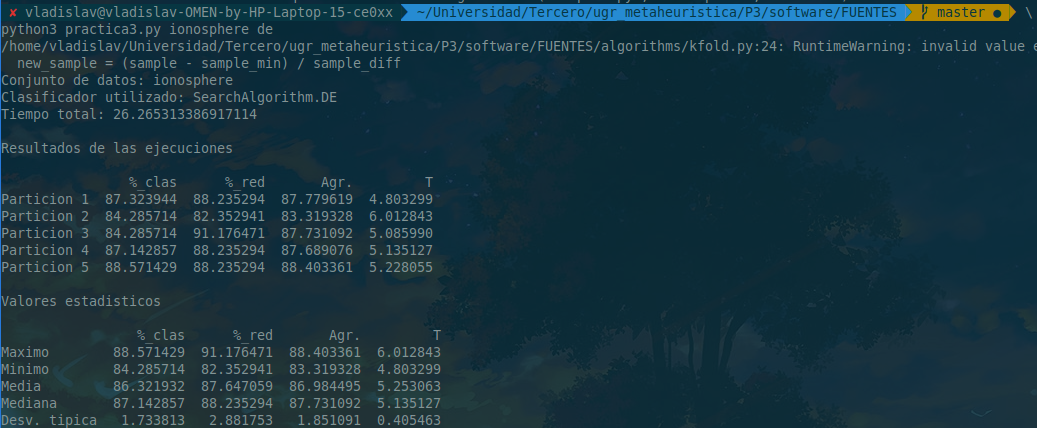
\includegraphics[scale=0.4]{img/out_example.png}
\caption{Ejemplo de salida de la ejecución con los datos \textbf{ionosphere} y la Evolución Diferencial con
\textit{current-to-best/1}.}
\end{figure}

\newpage

\section{Análisis de resultados y experimentación}

\subsection{Descripción de los casos del problema}

Para analizar el rendimiento de los algoritmos, se han realizado pruebas sobre 3 conjuntos de datos:

\begin{itemize}[label=\textbullet]
	\item \textbf{Colposcopy}: Conjunto de datos de colposcopias adquirido y anotado por médicos profesionales del Hospital
	Universitario de Caracas. Las imágenes fueron tomadas al azar de las secuencias colposcópicas. 287 ejemplos con 62
	características que deben ser clasificados en 2 clases.
	\item \textbf{Ionosphere}: Conjunto de datos de radar que fueron recogidos por un sistema en \textit{Goose Bay},
	Labrador. 352 ejemplos con 34 características que deben ser clasificados en 2 clases.
	\item \textbf{Texture}: Conjunto de datos de extracciones de imágenes para distinguir entre 11 texturas diferentes
	(césped, piel de becerro prensada, papel hecho a mano, rafia en bucle a una pila alta, lienzo de algodón,...). 550
	ejemplos con 40 características que deben ser clasificados en 11 clases.
\end{itemize}

\subsection{Análisis de los resultados}

Se han realizado distintas ejecuciones con los datos para cada uno de los algoritmos. Cada conjunto de datos se ha dividido
con una función de \textbf{sklearn}, y se han mezclado con la \textbf{semialla aleatoria} 40. Antes de ejecutar cada uno de los
algoritmos con la primera partición de datos se ha fijado como \textbf{semilla} el valor 8912374 (la misma que la práctica 
anterior para realizar un análisis más justo, ya que si no podría pasar que alguno de los nuevos algoritmos es mejor). Ambas 
están fijadas en el código y se pueden comprobar. Es muy importante destacar que todas las gráficas que se vean proceden de
la primera partición de cada conjunto de datos, con el objetivo de el análisis sea sobre los mismos datos, en vez de sobre
diferentes particiones.

A continuación se muestran los resultados obtenidos para cada algoritmo y para cada uno de los conjuntos de datos, rescatando
las tablas de la práctica anterior. Se han medido los valores de tasa de clasificación, tasa de reducción, agrupación (función
objetivo) y tiempo que ha tardado (en segundos). Además se ofrece información extra sobre los valores máximo, mínimo, medio,
mediana y desviación típica de cada uno de los datos, para poder comparar los datos más fácilmente. Y, como extra, se ha añadido
una tabla en la que aparecen los valores medios de cada algoritmo, para facilitar la comparación. Estas tablas se pueden ver
a continuación:

\begin{table}[H]
\resizebox{\columnwidth}{!}{%
\begin{tabular}{c|c|c|c|c|c|c|c|c|c|c|c|c|}
\cline{2-13}
\multicolumn{1}{l|}{}                       & \multicolumn{4}{c|}{\textbf{Colposcopy}}                                                   & \multicolumn{4}{c|}{\textbf{Ionosphere}}                                                   & \multicolumn{4}{c|}{\textbf{Texture}}                                                      \\ \cline{2-13} 
\multicolumn{1}{l|}{}                       & \textit{\textbf{\%\_clas}} & \textit{\textbf{\%red}} & \textit{\textbf{Agr.}} & \textbf{T} & \textit{\textbf{\%\_clas}} & \textit{\textbf{\%red}} & \textit{\textbf{Agr.}} & \textbf{T} & \textit{\textbf{\%\_clas}} & \textit{\textbf{\%red}} & \textit{\textbf{Agr.}} & \textbf{T} \\ \hline
\multicolumn{1}{|c|}{\textbf{Partición 1}}  & 79,66                      & 0                       & 39,83                  & 0,00049    & 85,92                      & 0                       & 42,96                  & 0,00045    & 91,82                      & 0                       & 45,91                  & 0,00056    \\ \hline
\multicolumn{1}{|c|}{\textbf{Partición 2}}  & 66,67                      & 0                       & 33,33                  & 0,00037    & 85,71                      & 0                       & 42,86                  & 0,00037    & 91,82                      & 0                       & 45,91                  & 0,00048    \\ \hline
\multicolumn{1}{|c|}{\textbf{Partición 3}}  & 71,93                      & 0                       & 35,96                  & 0,00035    & 88,57                      & 0                       & 44,29                  & 0,00036    & 93,64                      & 0                       & 46,82                  & 0,00044    \\ \hline
\multicolumn{1}{|c|}{\textbf{Partición 4}}  & 82,46                      & 0                       & 41,23                  & 0,00035    & 87,14                      & 0                       & 43,57                  & 0,00039    & 93,64                      & 0                       & 46,82                  & 0,00046    \\ \hline
\multicolumn{1}{|c|}{\textbf{Partición 5}}  & 73,68                      & 0                       & 36,84                  & 0,00035    & 84,29                      & 0                       & 42,14                  & 0,00039    & 90,91                      & 0                       & 45,45                  & 0,00049    \\ \hline
\multicolumn{1}{|c|}{\textbf{Media}}        & 74,88                      & 0                       & 37,44                  & 0,00038    & 86,33                      & 0                       & 43,16                  & 0,00039    & 92,36                      & 0                       & 46,18                  & 0,00049    \\ \hline
\multicolumn{1}{|c|}{\textbf{Máximo}}       & 82,46                      & 0                       & 41,23                  & 0,00049    & 88,57                      & 0                       & 44,29                  & 0,00048    & 93,64                      & 0                       & 46,82                  & 0,00056    \\ \hline
\multicolumn{1}{|c|}{\textbf{Mínimo}}       & 66,67                      & 0                       & 33,33                  & 0,00035    & 84,29                      & 0                       & 42,14                  & 0,00036    & 90,91                      & 0                       & 45,45                  & 0,00044    \\ \hline
\multicolumn{1}{|c|}{\textbf{Mediana}}      & 73,68                      & 0                       & 36,84                  & 0,00035    & 85,92                      & 0                       & 42,96                  & 0,00039    & 91,82                      & 0                       & 45,91                  & 0,00048    \\ \hline
\multicolumn{1}{|c|}{\textbf{Desv. Típica}} & 5,62                       & 0                       & 2,81                   & 0,000056   & 1,44                       & 0                       & 0,72                   & 0,000033   & 1,09                       & 0                       & 0,55                   & 0,00004    \\ \hline
\end{tabular}
}%
\caption{Resultados obtenidos por el algoritmo 1-NN en el problema del APC.}
\end{table}

\begin{table}[H]
\resizebox{\columnwidth}{!}{%
\begin{tabular}{c|c|c|c|c|c|c|c|c|c|c|c|c|}
\cline{2-13}
\multicolumn{1}{l|}{}                       & \multicolumn{4}{c|}{\textbf{Colposcopy}}                                                   & \multicolumn{4}{c|}{\textbf{Ionosphere}}                                                   & \multicolumn{4}{c|}{\textbf{Texture}}                                                      \\ \cline{2-13} 
\multicolumn{1}{l|}{}                       & \textit{\textbf{\%\_clas}} & \textit{\textbf{\%red}} & \textit{\textbf{Agr.}} & \textbf{T} & \textit{\textbf{\%\_clas}} & \textit{\textbf{\%red}} & \textit{\textbf{Agr.}} & \textbf{T} & \textit{\textbf{\%\_clas}} & \textit{\textbf{\%red}} & \textit{\textbf{Agr.}} & \textbf{T} \\ \hline
\multicolumn{1}{|c|}{\textbf{Partición 1}}  & 72,88                      & 29,03                   & 50,96                  & 0,04223180 & 87,32                      & 2,94                    & 45,13                  & 0,04617286 & 93,64                      & 7,50                    & 50,57                  & 0,09011912 \\ \hline
\multicolumn{1}{|c|}{\textbf{Partición 2}}  & 70,18                      & 25,81                   & 47,99                  & 0,03592849 & 91,43                      & 2,94                    & 47,18                  & 0,04701781 & 94,55                      & 15,00                   & 54,77                  & 0,08130646 \\ \hline
\multicolumn{1}{|c|}{\textbf{Partición 3}}  & 68,42                      & 48,39                   & 58,40                  & 0,03983450 & 91,43                      & 2,94                    & 47,18                  & 0,03659153 & 95,45                      & 7,50                    & 51,48                  & 0,08078218 \\ \hline
\multicolumn{1}{|c|}{\textbf{Partición 4}}  & 77,19                      & 64,52                   & 70,85                  & 0,03201556 & 90,00                      & 2,94                    & 46,47                  & 0,03484225 & 97,27                      & 5,00                    & 51,14                  & 0,08749294 \\ \hline
\multicolumn{1}{|c|}{\textbf{Partición 5}}  & 82,46                      & 29,03                   & 55,74                  & 0,03293490 & 84,29                      & 2,94                    & 43,61                  & 0,03472829 & 93,64                      & 2,50                    & 48,07                  & 0,09723902 \\ \hline
\multicolumn{1}{|c|}{\textbf{Media}}        & 74,23                      & 39,35                   & 56,79                  & 0,03658905 & 88,89                      & 2,94                    & 45,92                  & 0,03987055 & 94,91                      & 7,50                    & 51,20                  & 0,08738794 \\ \hline
\multicolumn{1}{|c|}{\textbf{Máximo}}       & 82,46                      & 64,52                   & 70,85                  & 0,04223180 & 91,43                      & 2,94                    & 47,18                  & 0,04701781 & 97,27                      & 15,00                   & 54,77                  & 0,09723902 \\ \hline
\multicolumn{1}{|c|}{\textbf{Mínimo}}       & 68,42                      & 25,81                   & 47,99                  & 0,03201556 & 84,29                      & 2,94                    & 43,61                  & 0,03472829 & 93,64                      & 2,50                    & 48,07                  & 0,08078218 \\ \hline
\multicolumn{1}{|c|}{\textbf{Mediana}}      & 72,88                      & 29,03                   & 55,74                  & 0,03592849 & 90,00                      & 2,94                    & 46,47                  & 0,03659153 & 94,55                      & 7,50                    & 51,14                  & 0,08749294 \\ \hline
\multicolumn{1}{|c|}{\textbf{Desv. Típica}} & 5,07                       & 14,91                   & 7,91                   & 0,00392631 & 2,75                       & 0,00                    & 1,37                   & 0,00553680 & 1,36                       & 4,18                    & 2,15                   & 0,00608498 \\ \hline
\end{tabular}
}%
\caption{Resultados obtenidos por el algoritmo \textit{RELIEF} en el problema del APC.}
\end{table}

\begin{table}[H]
\resizebox{\columnwidth}{!}{%
\begin{tabular}{c|c|c|c|c|c|c|c|c|c|c|c|c|}
\cline{2-13}
                                            & \multicolumn{4}{c|}{\textbf{Colposcopy}}                                                   & \multicolumn{4}{c|}{\textbf{Ionosphere}}                                                   & \multicolumn{4}{c|}{\textbf{Texture}}                                                      \\ \cline{2-13} 
                                            & \textit{\textbf{\%\_clas}} & \textit{\textbf{\%red}} & \textit{\textbf{Agr.}} & \textbf{T} & \textit{\textbf{\%\_clas}} & \textit{\textbf{\%red}} & \textit{\textbf{Agr.}} & \textbf{T} & \textit{\textbf{\%\_clas}} & \textit{\textbf{\%red}} & \textit{\textbf{Agr.}} & \textbf{T} \\ \hline
\multicolumn{1}{|c|}{\textbf{Partición 1}}  & 81,36                      & 83,87                   & 82,61                  & 2,47677159 & 88,73                      & 85,29                   & 87,01                  & 0,74606109 & 92,73                      & 77,50                   & 85,11                  & 0,81571221 \\ \hline
\multicolumn{1}{|c|}{\textbf{Partición 2}}  & 71,93                      & 82,26                   & 77,09                  & 2,88534594 & 88,57                      & 79,41                   & 83,99                  & 0,83731246 & 89,09                      & 85,00                   & 87,05                  & 0,86508775 \\ \hline
\multicolumn{1}{|c|}{\textbf{Partición 3}}  & 70,18                      & 82,26                   & 76,22                  & 2,59485793 & 80,00                      & 94,12                   & 87,06                  & 0,42965746 & 95,45                      & 82,50                   & 88,98                  & 1,02096820 \\ \hline
\multicolumn{1}{|c|}{\textbf{Partición 4}}  & 71,93                      & 82,26                   & 77,09                  & 2,90626860 & 88,57                      & 91,18                   & 89,87                  & 0,75856829 & 90,91                      & 85,00                   & 87,95                  & 1,56289935 \\ \hline
\multicolumn{1}{|c|}{\textbf{Partición 5}}  & 64,91                      & 75,81                   & 70,36                  & 2,81053543 & 85,71                      & 91,18                   & 88,45                  & 0,62555575 & 87,27                      & 82,50                   & 84,89                  & 1,22837043 \\ \hline
\multicolumn{1}{|c|}{\textbf{Media}}        & 72,06                      & 81,29                   & 76,68                  & 2,73475590 & 86,32                      & 88,24                   & 87,28                  & 0,67943101 & 91,09                      & 82,50                   & 86,80                  & 1,09860759 \\ \hline
\multicolumn{1}{|c|}{\textbf{Máximo}}       & 81,36                      & 83,87                   & 82,61                  & 2,90626860 & 88,73                      & 94,12                   & 89,87                  & 0,83731246 & 95,45                      & 85,00                   & 88,98                  & 1,56289935 \\ \hline
\multicolumn{1}{|c|}{\textbf{Mínimo}}       & 64,91                      & 75,81                   & 70,36                  & 2,47677159 & 80,00                      & 79,41                   & 83,99                  & 0,42965746 & 87,27                      & 77,50                   & 84,89                  & 0,81571221 \\ \hline
\multicolumn{1}{|c|}{\textbf{Mediana}}      & 71,93                      & 82,26                   & 77,09                  & 2,81053543 & 88,57                      & 91,18                   & 87,06                  & 0,74606109 & 90,91                      & 82,50                   & 87,05                  & 1,02096820 \\ \hline
\multicolumn{1}{|c|}{\textbf{Desv. Típica}} & 5,31                       & 2,81                    & 3,89                   & 0,16968432 & 3,35                       & 5,26                    & 1,95                   & 0,14206914 & 2,84                       & 2,74                    & 1,59                   & 0,27312796 \\ \hline
\end{tabular}
}%
\caption{Resultados obtenidos por el algoritmo BL en el problema del APC.}
\end{table}

\begin{table}[H]
\resizebox{\columnwidth}{!}{%
\begin{tabular}{c|c|c|c|c|c|c|c|c|c|c|c|c|}
\cline{2-13}
                                            & \multicolumn{4}{c|}{\textbf{Colposcopy}}                                 & \multicolumn{4}{c|}{\textbf{Ionosphere}}                        & \multicolumn{4}{c|}{\textbf{Texture}}                           \\ \cline{2-13} 
                                            & \textit{\textbf{\%\_clas}} & \textit{\textbf{\%red}} & \textit{\textbf{Agr.}} & \textbf{T} & \textit{\textbf{\%\_clas}} & \textit{\textbf{\%red}} & \textit{\textbf{Agr.}} & \textbf{T} & \textit{\textbf{\%\_clas}} & \textit{\textbf{\%red}} & \textit{\textbf{Agr.}} & \textbf{T} \\ \hline
\multicolumn{1}{|c|}{\textbf{Partición 1}}  & 77.97             & 72.58                   & 75.27         & 10.26      & 83.1              & 85.29          & 84.2          & 5.0        & 90.91             & 85.0           & 87.95         & 6.29       \\ \hline
\multicolumn{1}{|c|}{\textbf{Partición 2}}  & 66.67             & 72.58                   & 69.62         & 10.79      & 82.86             & 88.24          & 85.55         & 4.36       & 86.36             & 82.5           & 84.43         & 6.63       \\ \hline
\multicolumn{1}{|c|}{\textbf{Partición 3}}  & 78.95             & 59.68                   & 69.31         & 13.95      & 88.57             & 85.29          & 86.93         & 4.69       & 93.64             & 77.5           & 85.57         & 6.88       \\ \hline
\multicolumn{1}{|c|}{\textbf{Partición 4}}  & 77.19             & 74.19                   & 75.69         & 9.55       & 91.43             & 91.18          & 91.3          & 3.88       & 89.09             & 85.0           & 87.05         & 6.26       \\ \hline
\multicolumn{1}{|c|}{\textbf{Partición 5}}  & 71.93             & 72.58                   & 72.26         & 10.97      & 81.43             & 76.47          & 78.95         & 5.98       & 89.09             & 82.5           & 85.8          & 6.28       \\ \hline
\multicolumn{1}{|c|}{\textbf{Media}}        & 74.54             & 70.32                   & 72.43         & 11.1       & 85.48             & 85.29          & 85.39         & 4.78       & 89.82             & 82.5           & 86.16         & 6.47       \\ \hline
\multicolumn{1}{|c|}{\textbf{Máximo}}       & 78.95             & 74.19                   & 75.69         & 13.95      & 91.43             & 91.18          & 91.3          & 5.98       & 93.64             & 85.0           & 87.95         & 6.88       \\ \hline
\multicolumn{1}{|c|}{\textbf{Mínimo}}       & 66.67             & 59.68                   & 69.31         & 9.55       & 81.43             & 76.47          & 78.95         & 3.88       & 86.36             & 77.5           & 84.43         & 6.26       \\ \hline
\multicolumn{1}{|c|}{\textbf{Mediana}}      & 77.19             & 72.58                   & 72.26         & 10.79      & 83.1              & 85.29          & 85.55         & 4.69       & 89.09             & 82.5           & 85.8          & 6.29       \\ \hline
\multicolumn{1}{|c|}{\textbf{Desv. Típica}} & 4.63              & 5.36                    & 2.7           & 1.51       & 3.84              & 4.92           & 4.01          & 0.7        & 2.4               & 2.74           & 1.22          & 0.25       \\ \hline
\end{tabular}
}%
\caption{Resultados obtenidos por el AGG con cruce BLX-$\alpha$ en el problema del APC.}
\end{table}

\begin{table}[H]
\resizebox{\columnwidth}{!}{%
\begin{tabular}{c|c|c|c|c|c|c|c|c|c|c|c|c|}
\cline{2-13}
                                            & \multicolumn{4}{c|}{\textbf{Colposcopy}}                                 & \multicolumn{4}{c|}{\textbf{Ionosphere}}                        & \multicolumn{4}{c|}{\textbf{Texture}}                           \\ \cline{2-13} 
                                            & \textit{\textbf{\%\_clas}} & \textit{\textbf{\%red}} & \textit{\textbf{Agr.}} & \textbf{T} & \textit{\textbf{\%\_clas}} & \textit{\textbf{\%red}} & \textit{\textbf{Agr.}} & \textbf{T} & \textit{\textbf{\%\_clas}} & \textit{\textbf{\%red}} & \textit{\textbf{Agr.}} & \textbf{T} \\ \hline
\multicolumn{1}{|c|}{\textbf{Partición 1}}  & 81.36             & 58.06                   & 69.71         & 18.7       & 87.32             & 61.76          & 74.54         & 9.83       & 93.64             & 75.0           & 84.32         & 8.72       \\ \hline
\multicolumn{1}{|c|}{\textbf{Partición 2}}  & 73.68             & 51.61                   & 62.65         & 17.91      & 85.71             & 70.59          & 78.15         & 9.98       & 90.91             & 77.5           & 84.2          & 8.04       \\ \hline
\multicolumn{1}{|c|}{\textbf{Partición 3}}  & 66.67             & 54.84                   & 60.75         & 14.76      & 90.0              & 64.71          & 77.35         & 9.03       & 92.73             & 62.5           & 77.61         & 10.16      \\ \hline
\multicolumn{1}{|c|}{\textbf{Partición 4}}  & 78.95             & 54.84                   & 66.89         & 16.96      & 91.43             & 64.71          & 78.07         & 8.22       & 90.91             & 67.5           & 79.2          & 9.85       \\ \hline
\multicolumn{1}{|c|}{\textbf{Partición 5}}  & 71.93             & 48.39                   & 60.16         & 18.4       & 81.43             & 61.76          & 71.6          & 10.36      & 90.91             & 55.0           & 72.95         & 12.62      \\ \hline
\multicolumn{1}{|c|}{\textbf{Media}}        & 74.52             & 53.55                   & 64.03         & 17.35      & 87.18             & 64.71          & 75.94         & 9.48       & 91.82             & 67.5           & 79.66         & 9.88       \\ \hline
\multicolumn{1}{|c|}{\textbf{Máximo}}       & 81.36             & 58.06                   & 69.71         & 18.7       & 91.43             & 70.59          & 78.15         & 10.36      & 93.64             & 77.5           & 84.32         & 12.62      \\ \hline
\multicolumn{1}{|c|}{\textbf{Mínimo}}       & 66.67             & 48.39                   & 60.16         & 14.76      & 81.43             & 61.76          & 71.6          & 8.22       & 90.91             & 55.0           & 72.95         & 8.04       \\ \hline
\multicolumn{1}{|c|}{\textbf{Mediana}}      & 73.68             & 54.84                   & 62.65         & 17.91      & 87.32             & 64.71          & 77.35         & 9.83       & 90.91             & 67.5           & 79.2          & 9.85       \\ \hline
\multicolumn{1}{|c|}{\textbf{Desv. Típica}} & 5.2               & 3.29                    & 3.69          & 1.42       & 3.5               & 3.22           & 2.54          & 0.76       & 1.15              & 8.22           & 4.28          & 1.57       \\ \hline
\end{tabular}
}%
\caption{Resultados obtenidos por el AGG con cruce aritmético en el problema del APC.}
\end{table}


\begin{table}[H]
\resizebox{\columnwidth}{!}{%
\begin{tabular}{c|c|c|c|c|c|c|c|c|c|c|c|c|}
\cline{2-13}
                                            & \multicolumn{4}{c|}{\textbf{Colposcopy}}                                 & \multicolumn{4}{c|}{\textbf{Ionosphere}}                        & \multicolumn{4}{c|}{\textbf{Texture}}                           \\ \cline{2-13} 
                                            & \textit{\textbf{\%\_clas}} & \textit{\textbf{\%red}} & \textit{\textbf{Agr.}} & \textbf{T} & \textit{\textbf{\%\_clas}} & \textit{\textbf{\%red}} & \textit{\textbf{Agr.}} & \textbf{T} & \textit{\textbf{\%\_clas}} & \textit{\textbf{\%red}} & \textit{\textbf{Agr.}} & \textbf{T} \\ \hline
\multicolumn{1}{|c|}{\textbf{Partición 1}}  & 69.49             & 72.58                   & 71.04         & 11.01      & 88.73             & 91.18          & 89.95         & 5.58       & 88.18             & 80.0           & 84.09         & 8.03       \\ \hline
\multicolumn{1}{|c|}{\textbf{Partición 2}}  & 71.93             & 70.97                   & 71.45         & 11.7       & 85.71             & 88.24          & 86.97         & 6.71       & 85.45             & 75.0           & 80.23         & 7.94       \\ \hline
\multicolumn{1}{|c|}{\textbf{Partición 3}}  & 68.42             & 64.52                   & 66.47         & 13.99      & 81.43             & 82.35          & 81.89         & 8.23       & 94.55             & 85.0           & 89.77         & 6.83       \\ \hline
\multicolumn{1}{|c|}{\textbf{Partición 4}}  & 77.19             & 80.65                   & 78.92         & 10.92      & 80.0              & 85.29          & 82.65         & 5.73       & 94.55             & 67.5           & 81.02         & 10.15      \\ \hline
\multicolumn{1}{|c|}{\textbf{Partición 5}}  & 71.93             & 70.97                   & 71.45         & 11.41      & 84.29             & 79.41          & 81.85         & 6.69       & 91.82             & 77.5           & 84.66         & 8.06       \\ \hline
\multicolumn{1}{|c|}{\textbf{Media}}        & 71.79             & 71.94                   & 71.86         & 11.81      & 84.03             & 85.29          & 84.66         & 6.59       & 90.91             & 77.0           & 83.95         & 8.2        \\ \hline
\multicolumn{1}{|c|}{\textbf{Máximo}}       & 77.19             & 80.65                   & 78.92         & 13.99      & 88.73             & 91.18          & 89.95         & 8.23       & 94.55             & 85.0           & 89.77         & 10.15      \\ \hline
\multicolumn{1}{|c|}{\textbf{Mínimo}}       & 68.42             & 64.52                   & 66.47         & 10.92      & 80.0              & 79.41          & 81.85         & 5.58       & 85.45             & 67.5           & 80.23         & 6.83       \\ \hline
\multicolumn{1}{|c|}{\textbf{Mediana}}      & 71.93             & 70.97                   & 71.45         & 11.41      & 84.29             & 85.29          & 82.65         & 6.69       & 91.82             & 77.5           & 84.09         & 8.03       \\ \hline
\multicolumn{1}{|c|}{\textbf{Desv. Típica}} & 3.03              & 5.16                    & 4.0           & 1.13       & 3.1               & 4.16           & 3.26          & 0.94       & 3.59              & 5.79           & 3.37          & 1.07       \\ \hline
\end{tabular}
}%
\caption{Resultados obtenidos por el AGE con cruce BLX-$\alpha$ en el problema del APC.}
\end{table}

\begin{table}[H]
\resizebox{\columnwidth}{!}{%
\begin{tabular}{c|c|c|c|c|c|c|c|c|c|c|c|c|}
\cline{2-13}
                                            & \multicolumn{4}{c|}{\textbf{Colposcopy}}                                 & \multicolumn{4}{c|}{\textbf{Ionosphere}}                        & \multicolumn{4}{c|}{\textbf{Texture}}                           \\ \cline{2-13} 
                                            & \textit{\textbf{\%\_clas}} & \textit{\textbf{\%red}} & \textit{\textbf{Agr.}} & \textbf{T} & \textit{\textbf{\%\_clas}} & \textit{\textbf{\%red}} & \textit{\textbf{Agr.}} & \textbf{T} & \textit{\textbf{\%\_clas}} & \textit{\textbf{\%red}} & \textit{\textbf{Agr.}} & \textbf{T} \\ \hline
\multicolumn{1}{|c|}{\textbf{Partición 1}}  & 74.58             & 59.68                   & 67.13         & 15.52      & 85.92             & 61.76          & 73.84         & 10.09      & 95.45             & 72.5           & 83.98         & 9.33       \\ \hline
\multicolumn{1}{|c|}{\textbf{Partición 2}}  & 68.42             & 66.13                   & 67.28         & 13.6       & 87.14             & 64.71          & 75.92         & 11.17      & 90.0              & 75.0           & 82.5          & 9.81       \\ \hline
\multicolumn{1}{|c|}{\textbf{Partición 3}}  & 68.42             & 67.74                   & 68.08         & 14.62      & 90.0              & 73.53          & 81.76         & 8.93       & 89.09             & 70.0           & 79.55         & 9.6        \\ \hline
\multicolumn{1}{|c|}{\textbf{Partición 4}}  & 77.19             & 69.35                   & 73.27         & 12.62      & 85.71             & 64.71          & 75.21         & 11.07      & 82.73             & 70.0           & 76.36         & 10.9       \\ \hline
\multicolumn{1}{|c|}{\textbf{Partición 5}}  & 70.18             & 69.35                   & 69.77         & 11.34      & 84.29             & 70.59          & 77.44         & 11.03      & 91.82             & 72.5           & 82.16         & 10.52      \\ \hline
\multicolumn{1}{|c|}{\textbf{Media}}        & 71.76             & 66.45                   & 69.1          & 13.54      & 86.61             & 67.06          & 76.84         & 10.46      & 89.82             & 72.0           & 80.91         & 10.03      \\ \hline
\multicolumn{1}{|c|}{\textbf{Máximo}}       & 77.19             & 69.35                   & 73.27         & 15.52      & 90.0              & 73.53          & 81.76         & 11.17      & 95.45             & 75.0           & 83.98         & 10.9       \\ \hline
\multicolumn{1}{|c|}{\textbf{Mínimo}}       & 68.42             & 59.68                   & 67.13         & 11.34      & 84.29             & 61.76          & 73.84         & 8.93       & 82.73             & 70.0           & 76.36         & 9.33       \\ \hline
\multicolumn{1}{|c|}{\textbf{Mediana}}      & 70.18             & 67.74                   & 68.08         & 13.6       & 85.92             & 64.71          & 75.92         & 11.03      & 90.0              & 72.5           & 82.16         & 9.81       \\ \hline
\multicolumn{1}{|c|}{\textbf{Desv. Típica}} & 3.53              & 3.59                    & 2.29          & 1.47       & 1.92              & 4.32           & 2.72          & 0.86       & 4.16              & 1.87           & 2.68          & 0.59       \\ \hline
\end{tabular}
}%
\caption{Resultados obtenidos por el AGE con cruce aritmético en el problema del APC.}
\end{table}

\begin{table}[H]
\resizebox{\columnwidth}{!}{%
\begin{tabular}{c|c|c|c|c|c|c|c|c|c|c|c|c|}
\cline{2-13}
                                            & \multicolumn{4}{c|}{\textbf{Colposcopy}}                                 & \multicolumn{4}{c|}{\textbf{Ionosphere}}                        & \multicolumn{4}{c|}{\textbf{Texture}}                           \\ \cline{2-13} 
                                            & \textit{\textbf{\%\_clas}} & \textit{\textbf{\%red}} & \textit{\textbf{Agr.}} & \textbf{T} & \textit{\textbf{\%\_clas}} & \textit{\textbf{\%red}} & \textit{\textbf{Agr.}} & \textbf{T} & \textit{\textbf{\%\_clas}} & \textit{\textbf{\%red}} & \textit{\textbf{Agr.}} & \textbf{T} \\ \hline
\multicolumn{1}{|c|}{\textbf{Partición 1}}  & 69.49             & 85.48                   & 77.49         & 7.15       & 80.28             & 88.24          & 84.26         & 3.91       & 88.18             & 85.0           & 86.59         & 4.74       \\ \hline
\multicolumn{1}{|c|}{\textbf{Partición 2}}  & 68.42             & 80.65                   & 74.53         & 8.19       & 87.14             & 88.24          & 87.69         & 3.57       & 87.27             & 85.0           & 86.14         & 5.23       \\ \hline
\multicolumn{1}{|c|}{\textbf{Partición 3}}  & 80.7              & 83.87                   & 82.29         & 7.56       & 75.71             & 88.24          & 81.97         & 3.82       & 93.64             & 82.5           & 88.07         & 5.51       \\ \hline
\multicolumn{1}{|c|}{\textbf{Partición 4}}  & 84.21             & 83.87                   & 84.04         & 7.8        & 85.71             & 94.12          & 89.92         & 3.43       & 91.82             & 85.0           & 88.41         & 5.39       \\ \hline
\multicolumn{1}{|c|}{\textbf{Partición 5}}  & 78.95             & 83.87                   & 81.41         & 7.79       & 84.29             & 91.18          & 87.73         & 3.68       & 92.73             & 82.5           & 87.61         & 5.75       \\ \hline
\multicolumn{1}{|c|}{\textbf{Media}}        & 76.35             & 83.55                   & 79.95         & 7.7        & 82.63             & 90.0           & 86.31         & 3.68       & 90.73             & 84.0           & 87.36         & 5.32       \\ \hline
\multicolumn{1}{|c|}{\textbf{Máximo}}       & 84.21             & 85.48                   & 84.04         & 8.19       & 87.14             & 94.12          & 89.92         & 3.91       & 93.64             & 85.0           & 88.41         & 5.75       \\ \hline
\multicolumn{1}{|c|}{\textbf{Mínimo}}       & 68.42             & 80.65                   & 74.53         & 7.15       & 75.71             & 88.24          & 81.97         & 3.43       & 87.27             & 82.5           & 86.14         & 4.74       \\ \hline
\multicolumn{1}{|c|}{\textbf{Mediana}}      & 78.95             & 83.87                   & 81.41         & 7.79       & 84.29             & 88.24          & 87.69         & 3.68       & 91.82             & 85.0           & 87.61         & 5.39       \\ \hline
\multicolumn{1}{|c|}{\textbf{Desv. Típica}} & 6.28              & 1.58                    & 3.46          & 0.34       & 4.15              & 2.35           & 2.83          & 0.17       & 2.53              & 1.22           & 0.87          & 0.34       \\ \hline
\end{tabular}
}%
\caption{Resultados obtenidos por el AM con cruce BLX-$\alpha$ y Búsqueda Local sobre toda la población en el problema del
APC.}
\end{table}

\begin{table}[H]
\resizebox{\columnwidth}{!}{%
\begin{tabular}{c|c|c|c|c|c|c|c|c|c|c|c|c|}
\cline{2-13}
                                            & \multicolumn{4}{c|}{\textbf{Colposcopy}}                                 & \multicolumn{4}{c|}{\textbf{Ionosphere}}                        & \multicolumn{4}{c|}{\textbf{Texture}}                           \\ \cline{2-13} 
                                            & \textit{\textbf{\%\_clas}} & \textit{\textbf{\%red}} & \textit{\textbf{Agr.}} & \textbf{T} & \textit{\textbf{\%\_clas}} & \textit{\textbf{\%red}} & \textit{\textbf{Agr.}} & \textbf{T} & \textit{\textbf{\%\_clas}} & \textit{\textbf{\%red}} & \textit{\textbf{Agr.}} & \textbf{T} \\ \hline
\multicolumn{1}{|c|}{\textbf{Partición 1}}  & 72.88             & 83.87                   & 78.38         & 5.88       & 90.14             & 91.18          & 90.66         & 2.94       & 87.27             & 85.0           & 86.14         & 4.31       \\ \hline
\multicolumn{1}{|c|}{\textbf{Partición 2}}  & 71.93             & 83.87                   & 77.9          & 6.73       & 90.0              & 91.18          & 90.59         & 2.97       & 90.91             & 87.5           & 89.2          & 4.22       \\ \hline
\multicolumn{1}{|c|}{\textbf{Partición 3}}  & 70.18             & 83.87                   & 77.02         & 6.62       & 94.29             & 82.35          & 88.32         & 3.85       & 95.45             & 87.5           & 91.48         & 4.35       \\ \hline
\multicolumn{1}{|c|}{\textbf{Partición 4}}  & 75.44             & 80.65                   & 78.04         & 8.95       & 90.0              & 82.35          & 86.18         & 4.7        & 85.45             & 87.5           & 86.48         & 4.48       \\ \hline
\multicolumn{1}{|c|}{\textbf{Partición 5}}  & 59.65             & 82.26                   & 70.95         & 7.66       & 87.14             & 91.18          & 89.16         & 2.75       & 81.82             & 85.0           & 83.41         & 4.58       \\ \hline
\multicolumn{1}{|c|}{\textbf{Media}}        & 70.01             & 82.9                    & 76.46         & 7.17       & 90.31             & 87.65          & 88.98         & 3.44       & 88.18             & 86.5           & 87.34         & 4.39       \\ \hline
\multicolumn{1}{|c|}{\textbf{Máximo}}       & 75.44             & 83.87                   & 78.38         & 8.95       & 94.29             & 91.18          & 90.66         & 4.7        & 95.45             & 87.5           & 91.48         & 4.58       \\ \hline
\multicolumn{1}{|c|}{\textbf{Mínimo}}       & 59.65             & 80.65                   & 70.95         & 5.88       & 87.14             & 82.35          & 86.18         & 2.75       & 81.82             & 85.0           & 83.41         & 4.22       \\ \hline
\multicolumn{1}{|c|}{\textbf{Mediana}}      & 71.93             & 83.87                   & 77.9          & 6.73       & 90.0              & 91.18          & 89.16         & 2.97       & 87.27             & 87.5           & 86.48         & 4.35       \\ \hline
\multicolumn{1}{|c|}{\textbf{Desv. Típica}} & 5.45              & 1.29                    & 2.79          & 1.06       & 2.28              & 4.32           & 1.66          & 0.73       & 4.67              & 1.22           & 2.77          & 0.13       \\ \hline
\end{tabular}
}%
\caption{Resultados obtenidos por el AM con cruce BLX-$\alpha$ y Búsqueda Local sobre el mejor de la población en el problema
del APC.}
\end{table}

\begin{table}[H]
\resizebox{\columnwidth}{!}{%
\begin{tabular}{c|c|c|c|c|c|c|c|c|c|c|c|c|}
\cline{2-13}
                                            & \multicolumn{4}{c|}{\textbf{Colposcopy}}                                 & \multicolumn{4}{c|}{\textbf{Ionosphere}}                        & \multicolumn{4}{c|}{\textbf{Texture}}                           \\ \cline{2-13} 
                                            & \textit{\textbf{\%\_clas}} & \textit{\textbf{\%red}} & \textit{\textbf{Agr.}} & \textbf{T} & \textit{\textbf{\%\_clas}} & \textit{\textbf{\%red}} & \textit{\textbf{Agr.}} & \textbf{T} & \textit{\textbf{\%\_clas}} & \textit{\textbf{\%red}} & \textit{\textbf{Agr.}} & \textbf{T} \\ \hline
\multicolumn{1}{|c|}{\textbf{Partición 1}}  & 72.88             & 83.87                   & 78.38         & 5.88       & 90.14             & 91.18          & 90.66         & 2.94       & 87.27             & 85.0           & 86.14         & 4.31       \\ \hline
\multicolumn{1}{|c|}{\textbf{Partición 2}}  & 71.93             & 83.87                   & 77.9          & 6.73       & 90.0              & 91.18          & 90.59         & 2.97       & 90.91             & 87.5           & 89.2          & 4.22       \\ \hline
\multicolumn{1}{|c|}{\textbf{Partición 3}}  & 70.18             & 83.87                   & 77.02         & 6.62       & 94.29             & 82.35          & 88.32         & 3.85       & 95.45             & 87.5           & 91.48         & 4.35       \\ \hline
\multicolumn{1}{|c|}{\textbf{Partición 4}}  & 75.44             & 80.65                   & 78.04         & 8.95       & 90.0              & 82.35          & 86.18         & 4.7        & 85.45             & 87.5           & 86.48         & 4.48       \\ \hline
\multicolumn{1}{|c|}{\textbf{Partición 5}}  & 59.65             & 82.26                   & 70.95         & 7.66       & 87.14             & 91.18          & 89.16         & 2.75       & 81.82             & 85.0           & 83.41         & 4.58       \\ \hline
\multicolumn{1}{|c|}{\textbf{Media}}        & 70.01             & 82.9                    & 76.46         & 7.17       & 90.31             & 87.65          & 88.98         & 3.44       & 88.18             & 86.5           & 87.34         & 4.39       \\ \hline
\multicolumn{1}{|c|}{\textbf{Máximo}}       & 75.44             & 83.87                   & 78.38         & 8.95       & 94.29             & 91.18          & 90.66         & 4.7        & 95.45             & 87.5           & 91.48         & 4.58       \\ \hline
\multicolumn{1}{|c|}{\textbf{Mínimo}}       & 59.65             & 80.65                   & 70.95         & 5.88       & 87.14             & 82.35          & 86.18         & 2.75       & 81.82             & 85.0           & 83.41         & 4.22       \\ \hline
\multicolumn{1}{|c|}{\textbf{Mediana}}      & 71.93             & 83.87                   & 77.9          & 6.73       & 90.0              & 91.18          & 89.16         & 2.97       & 87.27             & 87.5           & 86.48         & 4.35       \\ \hline
\multicolumn{1}{|c|}{\textbf{Desv. Típica}} & 5.45              & 1.29                    & 2.79          & 1.06       & 2.28              & 4.32           & 1.66          & 0.73       & 4.67              & 1.22           & 2.77          & 0.13       \\ \hline
\end{tabular}
}%
\caption{Resultados obtenidos por el AM con cruce BLX-$\alpha$ y Búsqueda Local sobre un cromosoma aleatorio  de la población
en el problema del APC.}
\end{table}


\newpage

\begin{thebibliography}{5}

\bibitem{pykdtree}
Repositroio de GitHub de pykdtree.
\\\url{https://github.com/storpipfugl/pykdtree}

\bibitem{ckdtree}
Documentación de cKDTree.
\\\url{https://docs.scipy.org/doc/scipy/reference/generated/scipy.spatial.cKDTree.html}

\end{thebibliography}

\end{document}

